\documentclass{beamer}
\usepackage[utf8]{inputenc}
\usepackage{amsmath}
\usefonttheme[onlymath]{serif}

\renewcommand{\familydefault}{\sfdefault}

\title{Finite Element Method for 2D heat equation}
\author{Tianyuan Wu, Mengying Wu}
\institute{ShanghaiTech University}
\date{2020.11.26}

\begin{document}

\frame{\titlepage}

\begin{frame}
\frametitle{Overview}
\begin{enumerate}
    \item 2D heat equation
    \item FEM for 2D heat equation
    \item Mesh generation
    \item Performance evaluation \& comparison
\end{enumerate}
\end{frame}

\begin{frame}
    \frametitle{Goal}
    \begin{enumerate}
        \item A FEM solver for 2D heat equation (* implemented in both Python and C++)
        \item A mesh generating algorithm for given region $\Omega$
        \item Performance evaluation for our solver
        \item * Data visualization (rendering) by matplotlib (Python) or OpenGL (C++)
    \end{enumerate}
\end{frame}

\begin{frame}
    \frametitle{2D heat equation}
    Formula:
    $$\frac{\partial{T}}{\partial{t}} = \lambda(\frac{\partial {^2 T}}{\partial{x^2}} + \frac{\partial {^2 T}}{\partial{y^2}}) + f(x, y, t)$$
    where $x, y \in \Omega$, and $T$ is the function of $x$, $y$ and time $t$.\\
    Also define the Neumann boundary condition: 
    $$\frac{\partial{T}}{\partial{\vec{n}}}\big |_{\partial{\Omega_n}} = T_{n}$$
    And the Dirichlet boundary condition:
    $$T\big| _{\partial{\Omega_d}} = T_{d}$$
\end{frame}

\begin{frame}
    \frametitle{Time elapse}
    In this project, we'll use update time variable $t$ by finite difference method:
    \begin{equation}\nonumber
    \begin{aligned}
        & \frac{T(x,y, t_{n+1}) - T(x, y, t_{n})}{dt} =\\
        & \lambda(\frac{\partial {^2 T(x, y, n+1)}}{\partial{x^2}} + \frac{\partial {^2 T(x, y, n+1)}}{\partial{y^2}}) + f(x, y, t_{n+1})
    \end{aligned}
    \end{equation}
    Denote $\frac{\partial {^2 T(x, y, n)}}{\partial{x^2}} + \frac{\partial {^2 T(x, y, n)}}{\partial{y^2}}$ as $\Delta T_n$, 
    and rewrite this equation as:
    $$\frac{T_{n+1} - T_{n}}{dt} = \lambda \Delta T_{n+1} + f_{n+1}$$
    Hence:
    $$T_{n+1}(1 - \lambda dt\Delta T_{n+1}) = f_{n+1}dt + T_{n}$$
\end{frame}

\begin{frame}
    \frametitle{FEM method for heat equation}
    Denote:\\
    Nodes: $N = \{n_1, n_2,\ldots, n_k\}$\\
    Triangle Mesh: $M = \{m_1, m_2,\ldots,  m_p\}$
    Then we discrete this equation as:
    $$T_{sol} = T_{sol, d} + T_{rest}$$
    where $T_{sol, d}$ is to fit the dirichlet boundary condition.
\end{frame}

\begin{frame}
    \frametitle{FEM method for heat equation}
    Denote $\{\phi_1, \phi_2, \ldots, \phi_k\}$ as the basis
    The Galerkin discretation of this equation is:
    \begin{equation}\nonumber
    \begin{aligned}
        & \int\limits_\Omega T_{rest, n} \phi_j dx+(\int\limits_\Omega \nabla T_{rest, n} \cdot \nabla \phi_j dx) \cdot \lambda dt \\
        & = \int\limits_\Omega T_{rest, n-1}\phi_j dx+(\int\limits_{\partial\Omega_n} T_{rest, n}^{neum} \phi_jds)\cdot dt+(\int\limits_\Omega F_n \phi_j dx)\cdot dt
    \end{aligned}
    \end{equation}
\end{frame}

\begin{frame}
    \frametitle{FEM method for heat equation - Cont'd}
    $$T_{rest, t} = \sum_{i=1}^{k}\alpha_i\phi^{i}_{t}$$
    Let $Tri$ denote the triangle mesh, hence we can construct the mass matrix
    $$M_{ij} = \sum\limits_{A\in Tri} \int\limits_A \phi_i  \phi_j dx$$, 
    coefficient matrix 
    $$A_{ij} = \int\limits_\Omega\nabla \phi_i \cdot \nabla \phi_j dx$$
    Hence we can get the matrix form of this equation
    \begin{equation}\nonumber
    \begin{aligned}
    & (Adt+M)T_{rest,n} = MT_{rest,n-1} \\
    & +(\int\limits_{\partial\Omega_n} T_{rest, n}^{neum} \phi_jds)\cdot dt+(\int\limits_\Omega F_n \phi_j dx)\cdot dt
    \end{aligned}
    \end{equation}
\end{frame}

\begin{frame}
    \frametitle{Triangle mesh}
    The triangle mesh $\phi_i(x, y)$ is shown in the following figure
    \begin{figure}[H]
        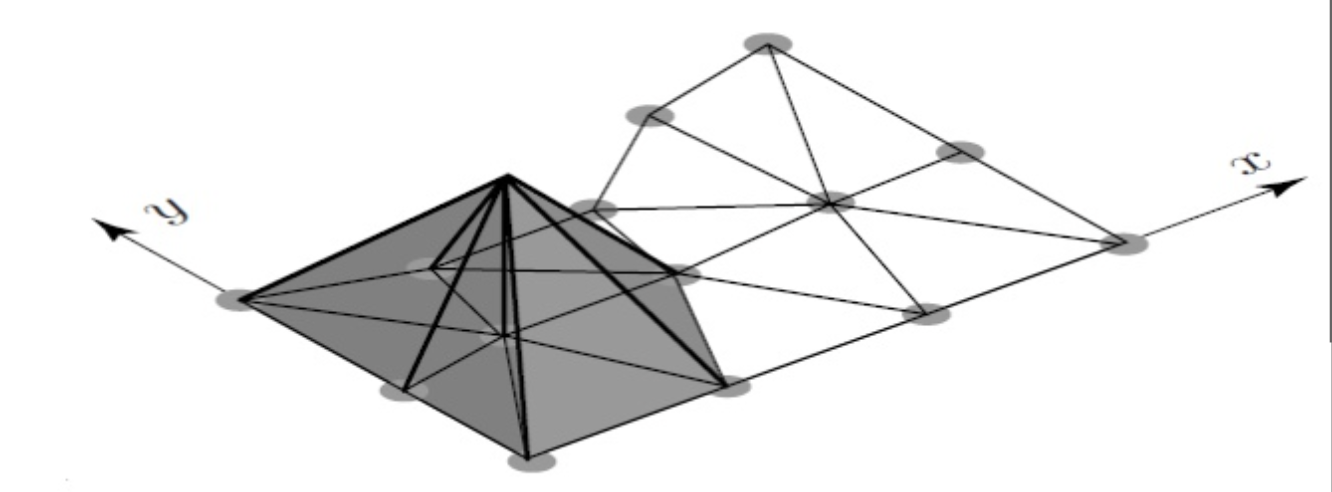
\includegraphics[scale=0.4]{mesh.png}
    \end{figure}
    Hence we can discrete the temperature function $T$ as 
    $$T_{rest, t} = \sum_{i=1}^{k}\alpha_i\phi^{i}_{t}$$
\end{frame}

\begin{frame}
    \frametitle{Mesh generation}
    \begin{enumerate}
        \item Regular region: Simple to implement
        \item Irregular region: Maybe we can refer to Delaunay triangulation, or using KD Tree
    \end{enumerate}
\end{frame}

\begin{frame}
    \frametitle{Performance evaluation \& comparison}
    \begin{enumerate}
        \item Evaluation of different mesh size / number of triangles
        \item Comparison between different implementations (Python vs. C++)
        \item Evaluation of different initial conditions, boundary conditions
    \end{enumerate}
\end{frame}

\begin{frame}
    {\centering\begin{center}
            \bf \Huge  Thanks!
        \end{center} }
\end{frame}

\end{document}
